\chapter{Balance de carga en SPS}
\label{cap:estadoDelArte}

\section{Perspectivas de balance de carga}
\label{sec:perspectivasBC}
Dentro de la literatura se han encontrado distintas perspectivas al problema de balance de carga en un SPS (Sistema de Procesamiento de \textsl{Streaming}), las cuales consideran los recursos físicos o lógicos como problemas de la sobrecarga del sistema.

\subsection{Recursos físicos}
\label{subsec:recFisicosBC}
En esta perspectiva se toma en consideración la sobrecarga del sistema dado las limitantes físicas que éste posea, ya sea por condiciones de los recursos disponibles o por el ambiente de desarrollo. Para esto, se consideran distintos parámetros como umbrales, los cuales si son sobrepasados debe aplicarse alguna estrategia para aliviar la carga del sistema. Estos umbrales pueden ser el nivel SLO, porcentaje de CPU utilizada o disponibilidad de la memoria \citep{Dong06schedulingalgorithms}.

Una de las soluciones con la perspectiva anterior es el Borealis \citep{XingZH05}, donde considera la cantidad de carga de los nodos en ventanas de tiempo determinadas, las cuales serán manejadas por un coordinador centralizado. Por lo que este coordinador estará encargada de analizar los recursos del sistema, y en caso de sobrepase el umbral propuesto, se deberán emigrar los operadores que estén en ese nodo, para luego ser enviados a otro nodo candidato con menor cantidad de carga. Para elegir al nodo candidato, se realizó una análisis de la cantidad de correlación que existe entre el operador y el nodo candidato, de esta manera, no necesariamente iba a ser enviado a otro nodo con menor sobrecarga, sino también a uno que posea menor cantidad de mensajes. Dentro de los problemas que pueden existir en el sistema es la conexión entre los distintos nodos, por lo que para las pruebas se consideró un buen ancho de banda, de tal manera que aparente una red sin limitaciones de recursos.

Otra de las soluciones que se han propuesto es lo realizado por Flood \citep{Alves2010flood}, el cual es un DPS (\textit{Distributed data stream processing}) que considera ciertos factores físicos para agregar o eliminar máquinas virtuales que se provee del \textit{Infrastructure-as-Service}, como Amazon EC2. Para esto, se posee un administrador que considera las estadísticas en tiempo de ejecución como la cantidad de CPU utilizada, latencia o memoria disponible, las cuales considera para ver en que rango está de los umbrales establecidos, y posteriormente agregar o eliminar recursos de manera elástica.

\subsection{Recursos lógicos}
\label{subsec:recLogicosBC}
%A diferencia de la física, aquí se consideran los componentes lógicos del sistema, como por ejemplo, una sobrecarga en algún operador. De esta manera, en las distintas soluciones se pueden encontrar soluciones en cuanto a la carga existente en el operador o la cantidad de cola que posea, de tal manera, que estos sean los umbrales a considerar para generar una mejora en el sistema.

A diferencia de la física, en esta perspectiva se consideran los componentes lógicos del sistema, como la carga de un operador. Por lo que las distintas soluciones que se presentan, analizan la componentes como el flujo de datos o el tamaño de la cola de un operador, tomando esos parámetros como umbrales en los algoritmos implementados para realizar mejoras en el sistema.

% Enfoques de la perspectiva lógica

Dado esta perspectiva, se han presentando dos tipos de enfoques: el estático y el dinámico \citep{Gupta99loadsharing}. El primer enfoque está centrado en un modelo definido y fijo antes de la inicialización del sistema, sin considerar el estado del sistema. En cambio, el segundo enfoque está basado en un modelo que analizará el sistema según su estado en el transcurso de su ejecución.

%El primer enfoque se centra en la confección de un modelo definido y fijo antes de iniciar el sistema y que no varía en el tiempo. En cambio, el segundo se basa en la adaptación del sistema según su estado en tiempo de ejecución.

\subsection{Enfoque estático}
\label{subsec:enfoqueEstaticoBC}
Este enfoque se ha implementando en distintos sistemas de procesamiento de \textsl{stream}, donde no se depende del estado del sistema \citep{stormtwitter, s4}. De esta manera, no existe una interrupción en la ejecución o un cambio debido al estado del sistema \citep{CasavantK88}. Por lo tanto, no se considera variables como la carga o cola del operador, sólo se aplican técnicas que administren el flujo de los datos en el sistema.

%\textsl{Storm} utiliza la técnica de distribución de operadores según alguna política, tomando el enfoque estático \citep{stormtwitter}. El sistema configura el número de operadores que son necesarios para realizar una tarea, para que después estos sean repartidos en los distintos nodos disponibles según la política de \textit{Shuffle grouping}. Esta técnica basada en algoritmos de planificación \citep{bookScheduling}, consiste en distribuir los operadores en los distintos nodos utilizando una planificación \textsl{Round-Robin}, de tal manera que la cantidad de operadores sea uniforme en los nodos del sistema \citep{bookstorm}.

\textsl{Storm} utiliza distintas técnicas de distribución de las tuplas en los operadores según la política que se desee, todas tomando el enfoque estático \citep{stormtwitter}. Dentro de las políticas que existen son \textit{Shuffle grouping}, \textit{Fields grouping}, \textit{Partial Key grouping}, \textit{All grouping}, \textit{Global grouping}, \textit{None grouping}, \textit{Direct grouping} y \textit{Local grouping}.

La política de \textit{Shuffle grouping} se enfoca en distribuir las tuplas de forma homogéneas en los $n$ operadores que se encuentren en el grafo, utilizando la planificación \textit{Round-Robin} \citep{bookScheduling}, de esta manera la cantidad de tuplas se distribuye de forma homogénea en el sistema. Una de las principales fallas es que la tasa de procesamiento de las tuplas no siempre es la misma, por lo tanto puede existir una sobrecarga en un operador que le llegue mayor cantidad de tuplas con un mayor tiempo de procesamiento. Otra de las políticas muy utilizadas es \textit{Fields grouping}, la cual determina ciertas llaves a un operador determinado, es decir, si la llave fueran palabras desde una letra hasta otra letra serán procesadas por cierto operado. Si bien genera un determinismo en el procesamiento de las llaves, puede existir una sobrecarga de un operador, debido que una llave se repite con mayor frecuencia que otras \citep{bookstorm}.

%Otra técnica es el uso de la función \textsl{hash} \citep{RogawayS04} para distribuir los operadores en el grafo, como lo planteado en S4 \citep{s4yahoo}. Esto consiste en aplicar lo anterior a algún atributo del evento, mapeando el evento al operador que corresponda de los $n$ operadores disponibles según el valor de la función. Cabe destacar que si no existe un operador mapeado con la imagen de la función, el sistema clona uno existente evaluando el nuevo con la imagen de la función como identificador. De esta manera, esta técnica provee dinamicidad respecto a la cantidad de operadores en el sistema.

Por otra parte, se encuentra el funcionamiento de S4, cuya política es similar a la de \textit{Fields grouping} de Storm, la diferencia es que un operador no le corresponde un conjunto de llaves, sino que posee una llave única. Esto quiere decir que cada llave se le asigna un operador, y en caso de no existir un operador para el valor de esa llave, se creará un nuevo operador para esa llave. Debido a la infinidad de combinaciones en la llave, S4 recomienda aplicar una función \textit{hash} \citep{RogawayS04}, de esta manera el valor de la función determina el operador que procesará el dato y disminuirá la cantidad de operadores que deben estar disponibles. Esta técnica provee dinamismo en la cantidad de operadores en el sistema, pero al igual que la \textit{Fields grouping} puede sobrecargar un operador, debido que una llave posee mayor frecuencia que las otras.

Una ventaja del enfoque estático es el bajo costo de la implementación de los métodos, lo cual es beneficioso para sistemas con bajos recursos. Por otra parte, una desventaja existente es la sobrecarga de un nodo u operador, debido que no asegura que la cantidad de flujo sea repartido de forma homogénea. Si bien, no es una solución óptima, es un buen complemento para un modelo con el enfoque dinámico.

\subsection{Enfoque dinámico}
\label{subsec:enfoqueDinamicoBC}

%Este enfoque está basado en el estado del sistema, donde según las variables y estado de cada uno de sus atributos, genera una acción en el sistema \citep{CasavantK88}. Esto significa que si el sistema posee alguna anomalía, como una sobrecarga en un operador o latencia entre distintos nodos, se realiza un cambio en el sistema, con el fin de solucionar estos problemas. Para poder dar una solución al problema de sobrecarga, se pueden utilizar dos tipos de modelos: reactivo y predictivo.

Este enfoque está basado en el estado del sistema, siendo esto el parámetro para optimizar el rendimiento del sistema \citep{CasavantK88}. Esto significa que si el sistema le surge una anomalía, como una sobrecarga o latencia entre nodos, es necesario realizar un cambio en el sistema, con el fin de solucionar estos problemas. Por lo que para solucionar estos problemas, se consideran dos modelos: el reactivo y el predictivo.

\paragraph{Reactivo}

Este modelo está basado en la detección de sobrecargas en el sistema a través de un monitor \citep{GulisanoJPSV12}, el cual recibe periódicamente las variables de cada uno los operadores, y en caso que sobrepase un umbral, se aplica una técnica para aumentar el rendimiento bajo una métrica dada. El umbral puede estar basado en el tiempo de procesamiento, el tamaño de la cola u otra variable del operador \citep{BhuvanagiriGKS06}. Por ejemplo, para realizar una optimización en el rendimiento general del sistema, se considera la tasa de procesamiento de cada operador, por lo que en caso de existir congestión en un operador, se procede a realizar una paralelización del operador, de tal manera que exista un operador adicional que pueda recibir un flujo de datos y realizar la misma operación que el operador sobrecargado \citep{SchneiderAGBW09}.

Si bien estas soluciones en su mayoría son eficientes y poseen buen rendimiento, una de los principales problemas es que no analiza el comportamiento a futuro, debido que sólo analiza y resuelve la situación en el momento. Otro problema son los falsos positivos, debido que puede ser que en un momento exista un \textit{pick} de tráfico, pero esto era sólo un caso particular de un tiempo determinado, por lo que no era necesaria la mejora en el sistema.

\paragraph{Predictivo}

Este modelo está basado en modelos matemáticos que calculan o estiman el comportamiento a futuro del sistema, dada cierta información que se posee del sistema, como flujo entrante o carga de la CPU. Si bien no existen modelos predictivos para SPS, si los existen en otras áreas, como se explicó anteriormente en la subsección \ref{subSec:markovTrabajo}.

\section{Técnicas de balance de carga}
\label{sec:tecnicasBC}

Existen distintas técnicas de balance de carga que utilizan alguno de los dos modelos presentados anteriormente, las cuales están enfocadas en mejorar al rendimiento del sistema en caso de existir una sobrecarga \citep{HirzelSSGG13}. Dentro de las técnicas existentes se encuentran la planificación determinista \citep{XuCTS14, DongTS07}, \textit{load shedding} \citep{SheuC09}, migración \citep{XingZH05} y fisión \citep{GulisanoJPSV12, IshiiS11, GedikSHW14, FernandezMKP13}, si bien existen más, sólo se trataron estas porque se consideran las relevantes.

\subsection{Planificación determinista}
\label{sec:planificacionBC}
%La planificación determinista \citep{DongTS07} se centra en la planificación según los recursos y estados del sistema \textit{a priori} según alguna métrica \citep{XuCTS14}. Una métrica utilizada es la frecuencia de datos estimada en un nodo u operador \citep{Ganguly09}. Esta técnica se utiliza, por ejemplo, en \textit{StreamIt} \citep{ThiesKA02}. Una de las limitaciones es que si bien realiza una predicción determinista de la frecuencia, no necesariamente es correcta a futuro, por lo que no se puede predecir las tasas de tráfico en el transcurso del procesamiento, sino sólo estimarlas al comienzo de la ejecución del sistema.

La planificación determinista se centra en los conocimientos \textit{a priori} del sistema, esto significa que se consideran las variables del entorno que se poseen y respecto a esto se toma una decisión de como debe actuar el sistema. 

En el área de \textit{Stream processing}, se han realizado diferentes análisis de la estimación de frecuencia de \textit{data stream} en el sistema. Para poder realizar esto, se han considerado modelos matemáticos, tomando ventanas de tiempo de la frecuencia predicha y la real, para posteriormente generar con los datos una función que represente la frecuencia estimada del operador \citep{Ganguly09}. Pero no sólo se han considerado modelos matemáticos, sino también algoritmos que determinan la frecuencia del sistema dado el flujo de datos que se podría poseer \citep{BhuvanagiriGKS06}.

En otras áreas, como red de sensores, se utiliza esta técnica en el envío de estadísticas de dispositivos móviles, los cuales manejan información \textit{a priori} de donde están los sensores, de tal manera de determinar según la intensidad de la frecuencia, localización o clima, a dónde debe enviar la señal para que se recolecte la información correspondiente \citep{DongTS07}.

Una de las limitaciones es que si bien realiza una predicción determinista de la frecuencia, no necesariamente es correcta a futuro. Esto se debe a qué puede analizarse respecto al promedio, pero pueden surgir procesos anómalos en el transcurso de la ejecución que generará una sobrecarga en el sistema. Por lo tanto, la estimación al realizarse \textit{a priori}, sólo podrá considerar el inicio del sistema o ventanas de tiempo, por lo que puede existir un porcentaje de error considerable. Por otra parte, se considera que posee mejor rendimiento esta técnica si es que la frecuencia o función analizada es estacionaria.

\subsection{Load Shedding}
\label{sec:loadSheddingBC}
%Otra estrategia está orientada a descartar eventos de un operador sobrecargado, de tal manera de no generar colas en el sistema. Esta estrategia que si bien no está implementada en el sistema por defecto de S4, puede habilitarse \citep{s4}. Otro ejemplo, es la trasmisión de vídeo \textit{streaming}, donde se descartan los datos que son de baja calidad, para procesar en su mayoría información de alta calidad \citep{SheuC09}. Esta solución está pensada para disminuir la carga, perdiendo la exactitud de la información debido a la pérdida de datos. Por lo tanto existe una menor fiabilidad en el sistema en caso de realizar operaciones de transacción \citep{bookDistrSys}.

En los SPS también se encuentra la técnica de \textit{load shedding} o descarte de eventos, que consiste en descartar eventos del sistema en caso de existir un comportamiento anómalo, ya sea un máximo en la cantidad de la cola u otro factor como se puede apreciar en la Figura \ref{fig:loadShedding}. Por ejemplo, en la transmisión de \textit{video streaming}, al enviar el flujo de información existe un administrador que estará analizando el contenido a procesar, por lo que en caos de llegar datos de baja calidad, serán descartados por éste. De esta manera, al existir menor cantidad de datos que procesar, el sistema posee un mejor rendimiento, además de tener una mejor calidad en la visualización de los videos, dado que en su mayoría se procesan datos de alta calidad \citep{SheuC09}. 

\begin{figure}[!ht]
	\centering
	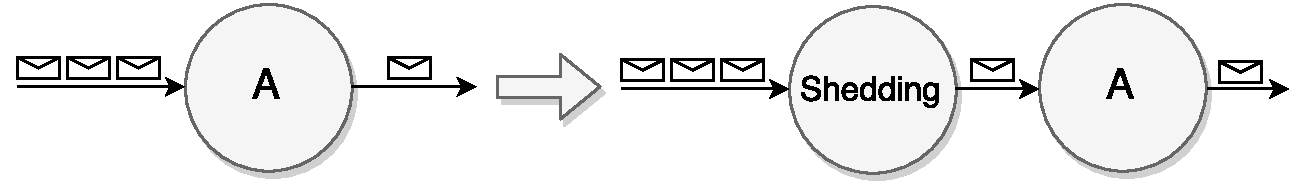
\includegraphics[scale=0.6]{images/LoadShedding.pdf}
	\caption{Load shedding en un SPS.}
	\label{fig:loadShedding}
\end{figure}

En el mundo de los SPS, varios poseen este tipo de estrategia, como por ejemplo S4 \citep{s4}, doonde se establece una cota superior de eventos en cola, y en caso que su cola sea igual al límite establecido, los eventos entrantes serán descartados. Otro sistema que aplica esta técnica es Aurora \citep{aurora}, el cual se basa en procesamiento de datos por ventanas de tiempo, por lo que en caso de existir una ventana de tiempo con una mayor cantidad de eventos de lo estipulado, se descartará el exceso de eventos.

Si bien esta técnica es simple y de bajo costo, siendo pensada para la disminución rápida de carga, existe una baja en la precisión y fiabilidad del procesamiento de los datos. Por ejemplo, en el caso de la transferencia de video no es trascendental, dado que son pocos los pixeles perdidos, pero en una recopilación y análisis de estadísticas, esto dará una menor precisión de los datos procesados por el sistema, dado que puede perderse información que indique comportamientos de los datos estudiados.

\subsection{Migración}
\label{sec:migracionBC}
%También se encuentra la migración, en el cual según el estado del sistema se migran los operadores de un nodo a otro. En \citep{XingZH05} se implementa   esta técnica, y si bien genera una menor carga en distintos nodos, produce un alto costo en la transferencia de los datos. Al realizar la transferencia de los datos, existe una menor tolerancia a fallos, a raíz de lo cual, se propone el uso de un búffer en el sistema, aumentando sus costos \citep{PittauACA07}.

La técnica de migración está basada en el traspaso de un operador de un nodo a otro, según el estado del sistema, como se puede apreciar en la Figura \ref{fig:migracion}. Si bien no existe alguna implementación que utilice los recursos lógicos, si existe una que utiliza los recursos físicos como es el caso de Borealis, el cual fue explicado anteriormente \citep{XingZH05}. Una de las principales críticas que se realiza a esta técnica, es la transferencia de datos, por lo que existe una menor tolerancia de fallos, por lo que se propone el uso de \textit{buffer} que tengan respaldos de la información, aumentando los costos del sistema \citep{PittauACA07}.

\begin{figure}[!ht]
	\centering
	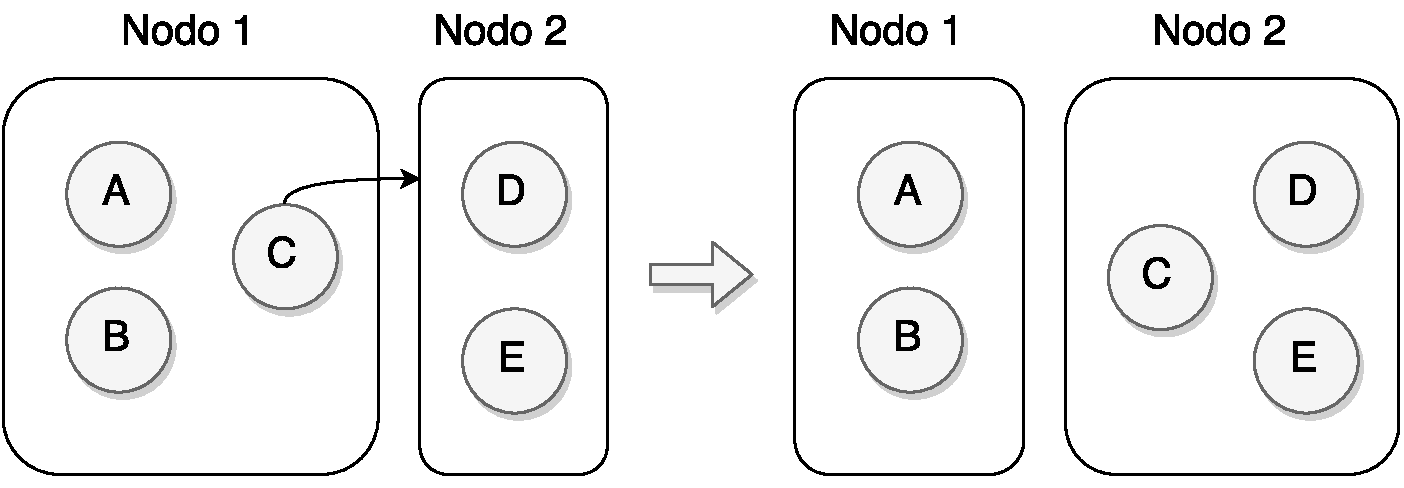
\includegraphics[scale=0.45]{images/Migracion.pdf}
	\caption{Técnia de migración en un SPS.}
	\label{fig:migracion}
\end{figure}

\subsection{Fisión}
\label{sec:fisionBC}

%Desde otra perspectiva, existen las técnicas de paralelización y replicación, las cuales se utilizan en caso de sobrepasar un umbral, el cual depende de la carga de un operador, nodo, entre otras variables. El primero consiste en paralelizar una tarea, la cual está determinada por un conjunto de operadores, en otro nodo físico \citep{IshiiS11}. En cambio, la replicación consiste en replicar un operador a nivel lógico del grafo \citep{MadsenTZ14}. Una de las características que existen en este tipo de soluciones es la elasticidad, que consiste en la capacidad de aumentar o disminuir la cantidad de operadores según la necesidad del sistema.

Otra técnica utilizada en el balance de carga es la fisión, o también llamada replicación, particionamiento o paralelismo, la cual consiste en crear una réplica paralela del operador, sin perder el funcionamiento y estado, en caso de existe una sobrecarga en el operador. En Figura \ref{fig:fision} se puede ver que existe un operador A, el cual en primera instancia tiene un flujo de entrada $q_1$ y flujo de salida $q_2$, pero debido a la sobrecarga del operador A, se crea dos operadores extras, los cuales pasarán por un \textit{Split} y posteriormente por un \textit{Merge}, que tendrán como función distribuir y juntar la información respectivamente. En ciertos SPS se posee el planteamiento que el \textit{split} y el \textit{merge} son operadores que deben ser realizados por el programador, y no de forma automática por el sistema, como S4 o Storm. Una de las características que se posee de esta técnica es la elasticidad del sistema, donde aumenta o disminuye la cantidad de operadores según la necesidad del sistema.

\begin{figure}[!ht]
	\centering
	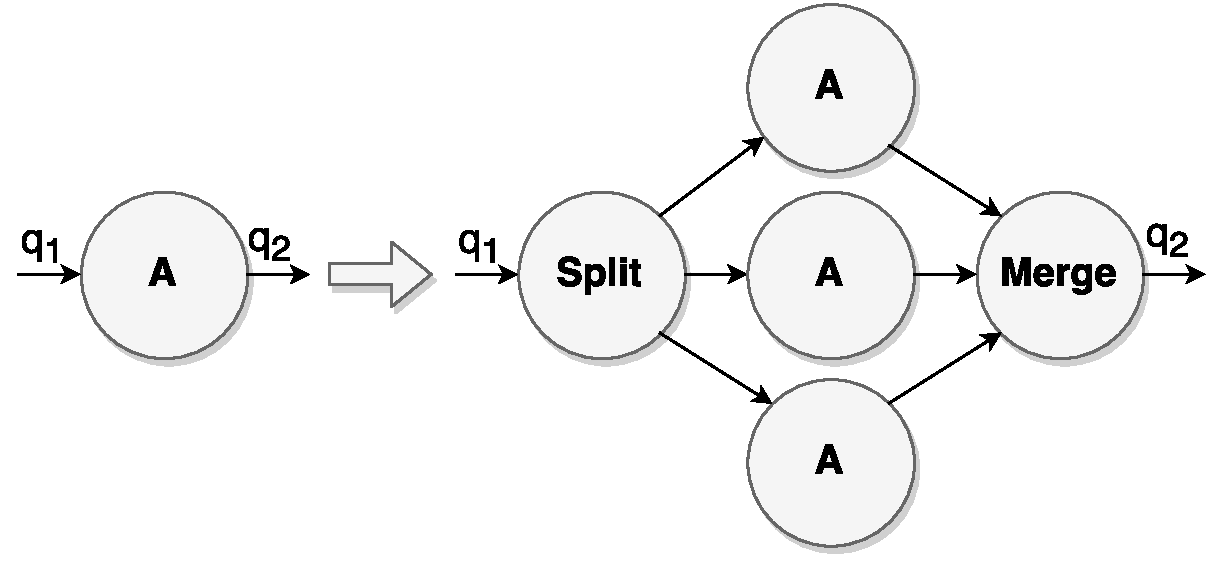
\includegraphics[scale=0.4]{images/Fision.pdf}
	\caption{Técnica de fisión en un SPS.}
	\label{fig:fision}
\end{figure}

%Una aplicación de la técnica de paralelización según el enfoque estático, es la paralelización de tareas de Storm \citep{stormtwitterdoc}, donde un conjunto de operadores realizan una tarea, indicado la cantidad de tareas que se desean ejecutar paralelamente en el sistema.

%Un ejemplo aplicado de esta técnica según el enfoque dińamico es StreamCloud \citep{GulisanoJPSV12}, que dada la cantidad de consultas que van llegando al sistema, se paralelizan las tareas existentes. Uno de los problemas que surge en estos casos son las operaciones con estado, como lo son los contadores o algoritmos de orden. La solución planteada es poseer un operador que realiza la tarea de \textit{merge}, que consiste en recibir las salidas de las tareas paralelas, agrupando los datos y proporcionando una salida según lo realizado por cada uno de las operaciones \citep{GedikSHW14}.

Una aplicación que aplica la técnica de fusión según el enfoque estático, es la paralelización de tareas de Storm \citep{stormtwitterdoc}, donde se indica la cantidad de operadores necesarios para realizar una tarea paralelamente. De esta manera, existe un proceso que está encargada de la tarea deseada, y $n$ hebras por la cantidad de operadores que se deseen.

Otro sistema que abarca esta técnica, utilizando el enfoque dinámico, es \textit{StreamCloud} \citep{GulisanoJPSV12}, donde según la cantidad de consultas realizadas al sistema, se aumenta o disminuye la cantidad de operadores que cumplan las tareas que se solicitan. Como se había mencionado anteriormente, existe un problema con la variable de distribución y unión de la información al replicar los operadores, este sistema propone que pueda resolver ciertas consultas el sistema y que de forma automática pueda realizar el proceso de \textit{split} y \textit{merge}, de tal manera de no tener problemas con los operadores con estado, como lo son los contadores y algoritmos de orden. Una de las características principales de este sistema, es aplicar el concepto de elasticidad, que aumenta y disminuye la cantidad de operadores según lo requerido por el sistema. Pero no sólo este tipo de sistemas aplica este método, también se puede ver otros trabajos como \citep{GedikSHW14, SchneiderAGBW09} que paralelizan las tareas de forma elástica, y con parámetros similares, sólo que su implementación es distinta.

El último trabajo a analizar según esta técnica es lo realizado por Fernández \citep{FernandezMKP13}, donde aplican fisión en el caso que exista un cuello de botella en un operador. Para la detección de estas situaciones, se posee un monitor, el cual está consultando en un período de tiempo corto el estado de cada uno de los operadores. De esta manera, se puede ver en cada operador si sobrepaso el umbral propuesto, que era en este caso la utilización de la CPU, se procede a replicar el operador sobrecargado. En la Figura \ref{fig:ejFision} se puede ver el caso de un simple sistema, en el cual el operador \textit{u} está enviado un flujo de datos al operador \textit{o}, hasta que en cierto momento el operador \textit{o} posee un cuello de botella y debe replicar, hasta que en la parte (c) denota que convergió y ya no es necesario más réplicas, pero con el transcurso del tiempo si fue necesario en el operador \textit{u}, por lo que se aplica la misma lógica descrita anteriormente con el operador \textit{o}.

\begin{figure}[!ht]
	\centering
	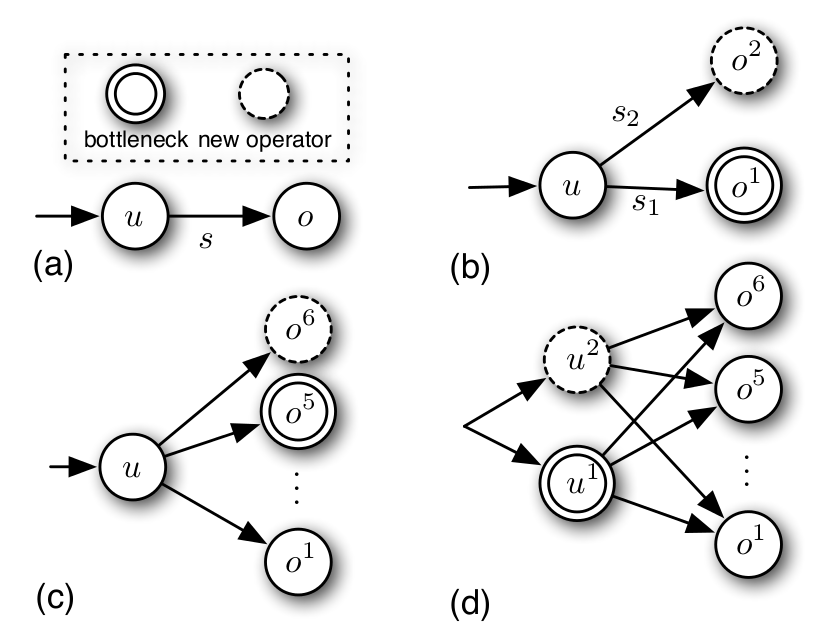
\includegraphics[scale=0.3]{images/EjFision.png}
	\caption{Ejemplo de replicación de los operadores \citep{FernandezMKP13}.}
	\label{fig:ejFision}
\end{figure}

%Por otra parte, se usa la técnica de replicación en una aplicación diseñada por Fernández \citep{FernandezMKP13}. Ésta está enfocada en la replicación de operadores, la cual se activa si se detecta un cuello botella en el procesamiento de los datos. Para la detección, existe un monitor que está recibiendo la carga de cada uno de los procesos, y si es sobrepasado el umbral, debe realizar una petición de replicación al operador sobrecargado.